\section{Documentation}

The development of our product started out with early-prototyping of the code and the individual components. Right after the research and initial analysis was completed, we started looking into running the individual components and searching for libraries that we needed to use. This helped us to identify problems like lack of documentation of LCD libraries for the Arduino MEGA board, which we considered to use at some point of our research. 


These smaller component-prototypes eventually became part of our prototype code.


The code for the prototype only works for the desired single-lock prototype. It can take any student card and associate it with a lock. But it will only store the card information when the lock is locked and delete the information when its unlocked. For future work we would use a centralized database to deal with multiple locks and cards.

\subsection{Code}

%---------------
	
\lstinputlisting[firstline=176, lastline=221, title=Prototype main loop]{./code/RFID_Prototype.cpp}

The main loop in the prototype code always checks if there is a new RFID tag read, or if a lock recently has been locked. If nothing is happening it will show the welcome screen. The main loop then has two main if statements. The first if statement checks if there is a RFID card read by the system and the second if statement checks if the sensor in the enclosure has been activated from the locking-peg.

 
If an RFID tag is read, it will check if it is a valid and connect it to a lock. If the card already is connected to a lock, the display will show a message to the user that the lock is unlocked and then unlocks the bicycle. 


If the sensor in the enclosure registers a new lock it will ask the user to scan their RFID tag/card. It will check if the card is valid or connected to another lock. It will do this for 30 seconds. If no valid RFID card is read in 30 seconds it will unlock the lock and display it to the user. The system has this feature in place to avoid people locking all the locks without associating them with a RFID card of some sort.


If a valid one is read it will display a message to the user that the system is locked and that their card is associated with that specific lock.


The main loop also addresses input errors. One is if at any time an RFID card is read that is invalid for this system and another is if the user is trying to lock the second bike lock with the same RFID card it will display an error message to the user.

\clearpage

%---------------

\lstinputlisting[firstline=223, lastline=233, title=Prototype sensorRead function]{./code/RFID_Prototype.cpp}

The function $sensorRead()$ checks if the lock has been locked. The end of the lock has a sensor and it will notify the program what lock has been locked. The program then goes to check for a new RFID tag for 30 seconds. If no RFID tag is scanned it will open the lock again. If a new RFID tag is entered it will change the number in the array $lockCheck[]$ from 0 to 1. So the program will ignore a previously locked lock.


%---------------


\lstinputlisting[firstline=414, lastline=428, title=Prototype lockLock function]{./code/RFID_Prototype.cpp}

Te function $lockLock()$ displays a message to the user that the lock is now locked and changes the array $lockCheck[0]=0$ to $lockCheck[0]=1$. That is done to prevent the system to check multiple times on the same lock that has been connected to an RFID tag.


%---------------

\lstinputlisting[firstline=280, lastline=298, title=Prototype getID function]{./code/RFID_V1.cpp}

The function $getID()$ checks if a new RFID tag is read by the RFID reader. If so it checks if the card is of the right type. It then writes it to the array $readCard[]$. It only stores 4 bytes of information, which is the ID of the card. The program ignores all of the other user data. In future versions we can hash the information, hashing is encrypting the data so that even if someone gets the data it is unusable.
  

%---------------

\lstinputlisting[firstline=435, lastline=449, title=Prototype checkTwo function]{./code/RFID_V1.cpp}

The function $checkTwo()$ compares two arrays together to see if they have the same data. The function compares the $storedCard[]$ array to $readCard[]$, to see if the card that is read is in the system or not. For future systems where there is more than one lock, it is also necessary to compare the pointer array $lock[]$ to $readCard[]$ and then open the connected lock to that RFID tag.

\clearpage

%---------------

\lstinputlisting[firstline=523, lastline=530, title=Prototype isMaster function]{./code/RFID_V1.cpp}

The function $isMaster$ only checks if the RFID tag that was read is the master card and uses the $checkTwo[]$ function to do that. Master card is used by the main user to help with the system if an error comes up or a card is lost.


%---------------

\subsection{Build}

The prototype case for the locking device is primarily built using plywood, a 12V solenoid, a mechanical relay, a switch and a Plexiglas cover.
 
\begin{figure}[H]
	\centering
	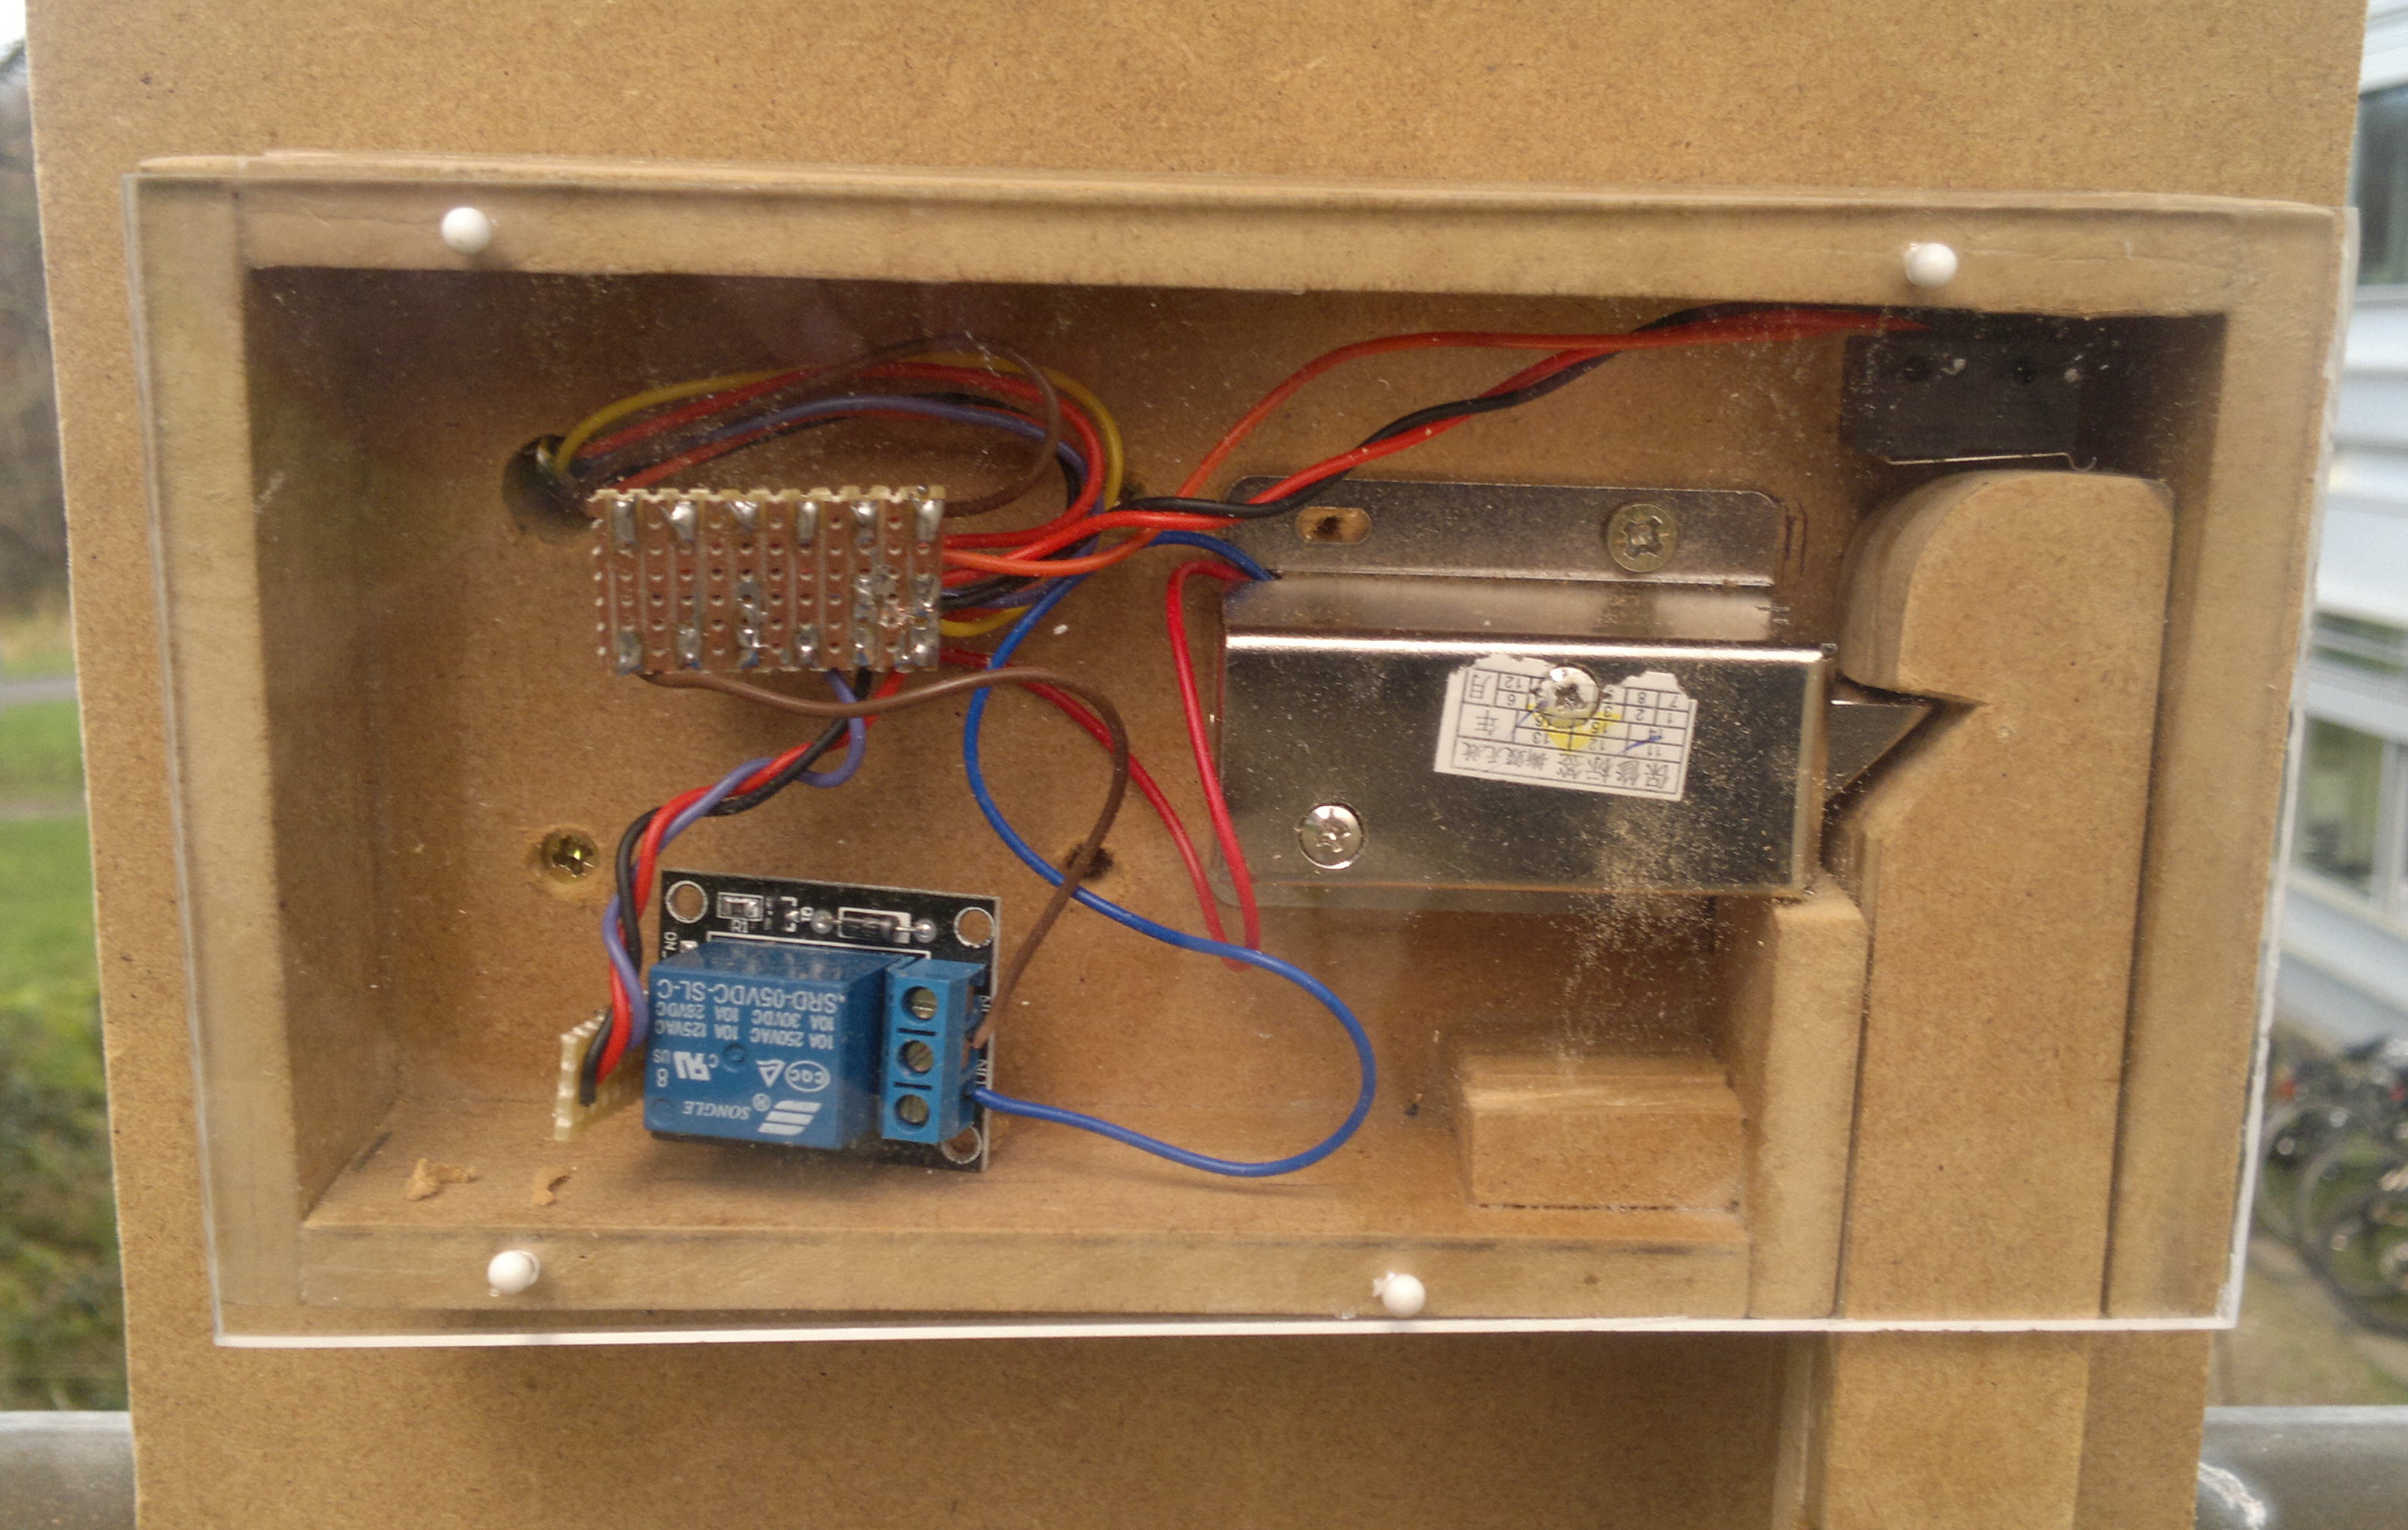
\includegraphics[width=0.6\textwidth]{images/desc/lock.jpg}
	\caption{Picture of lock}
	\label{fig.lock}
\end{figure}


The main prototype box contain an Arduino Uno development board (containing Atmel micro-comtroller), a RFID reader and a LCD 16x2 screen. They are placed in a ABS electrical box in which we have cut hole fitting the display. A RFID reader is located on the other side of the box, inside, under the label.

Both the locking enclosure and the case containing the micro-controller and electronic components are secured to a plywood wall and is mounted to the bicycle rack. The box containing the electronics is mounted on an extension that is tilted at an $45\,^{\circ}$ angle, making the display text more readable. The case containing the locking mechanism is mounted directly on the wall.

\begin{figure}[H]
	\centering
	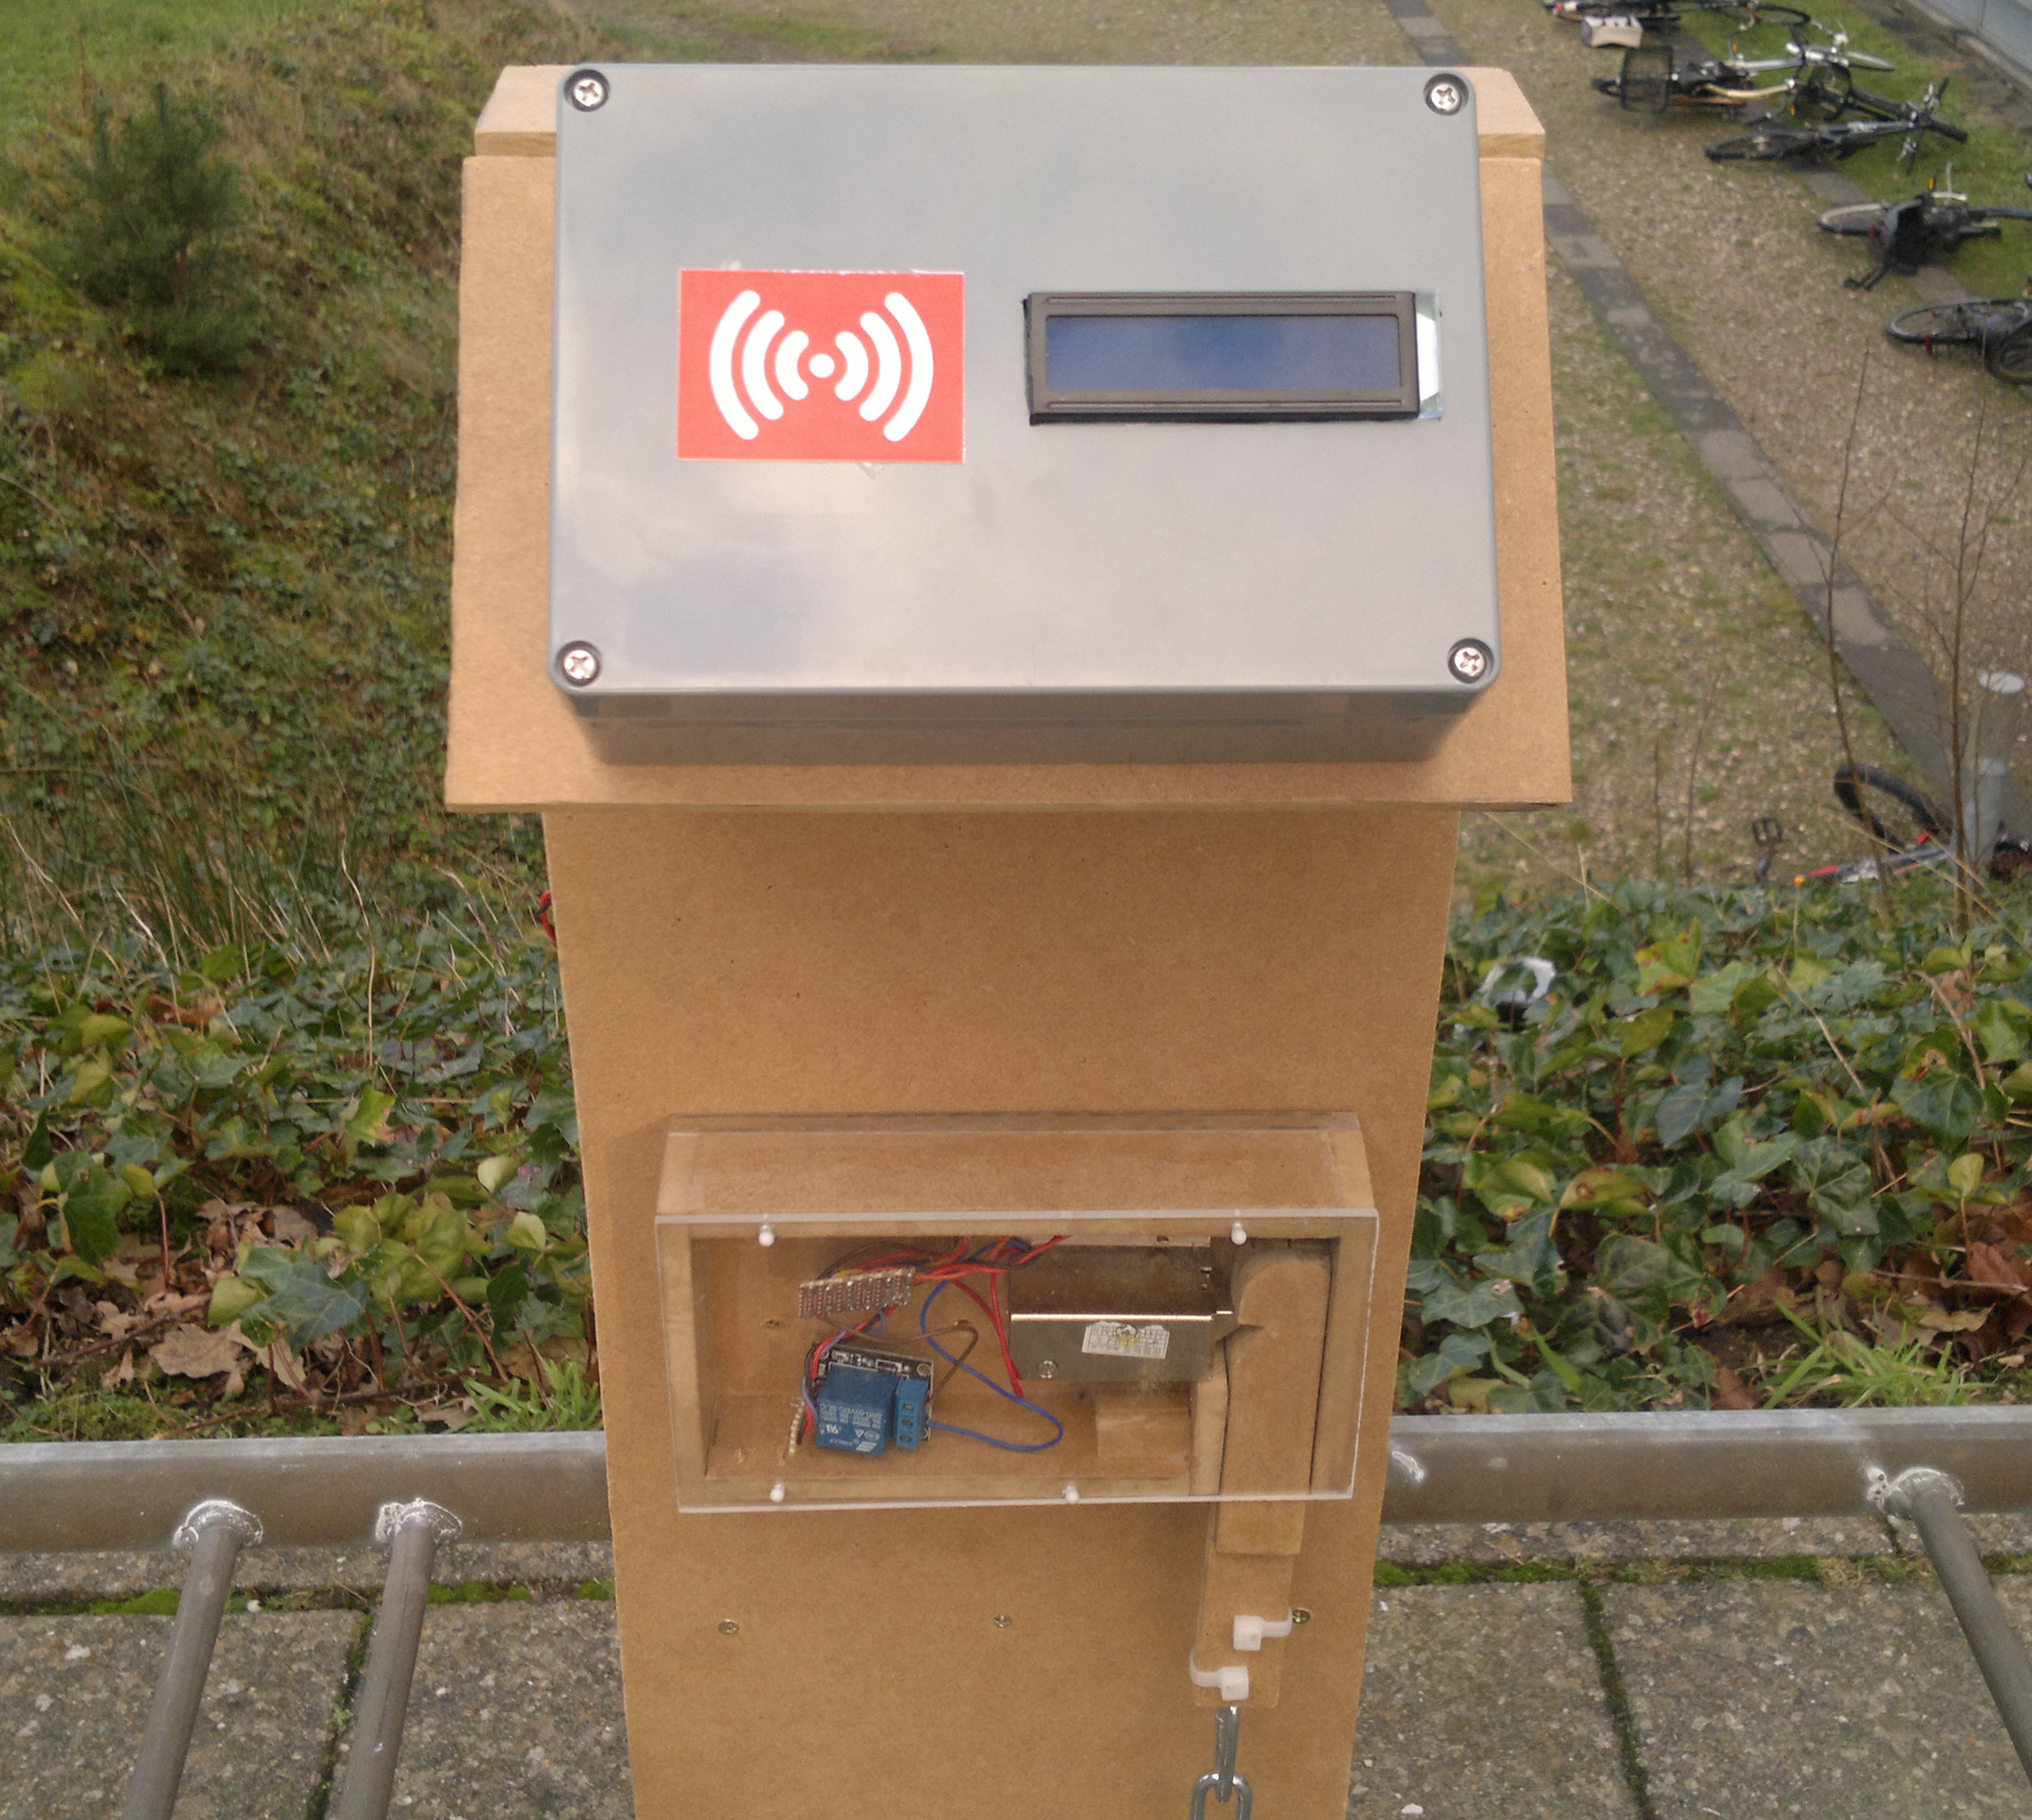
\includegraphics[width=0.6\textwidth]{images/desc/boxes.jpg}
	\caption{Picture of components}
	\label{fig.rack}
\end{figure}


\begin{figure}[H]
	\centering
	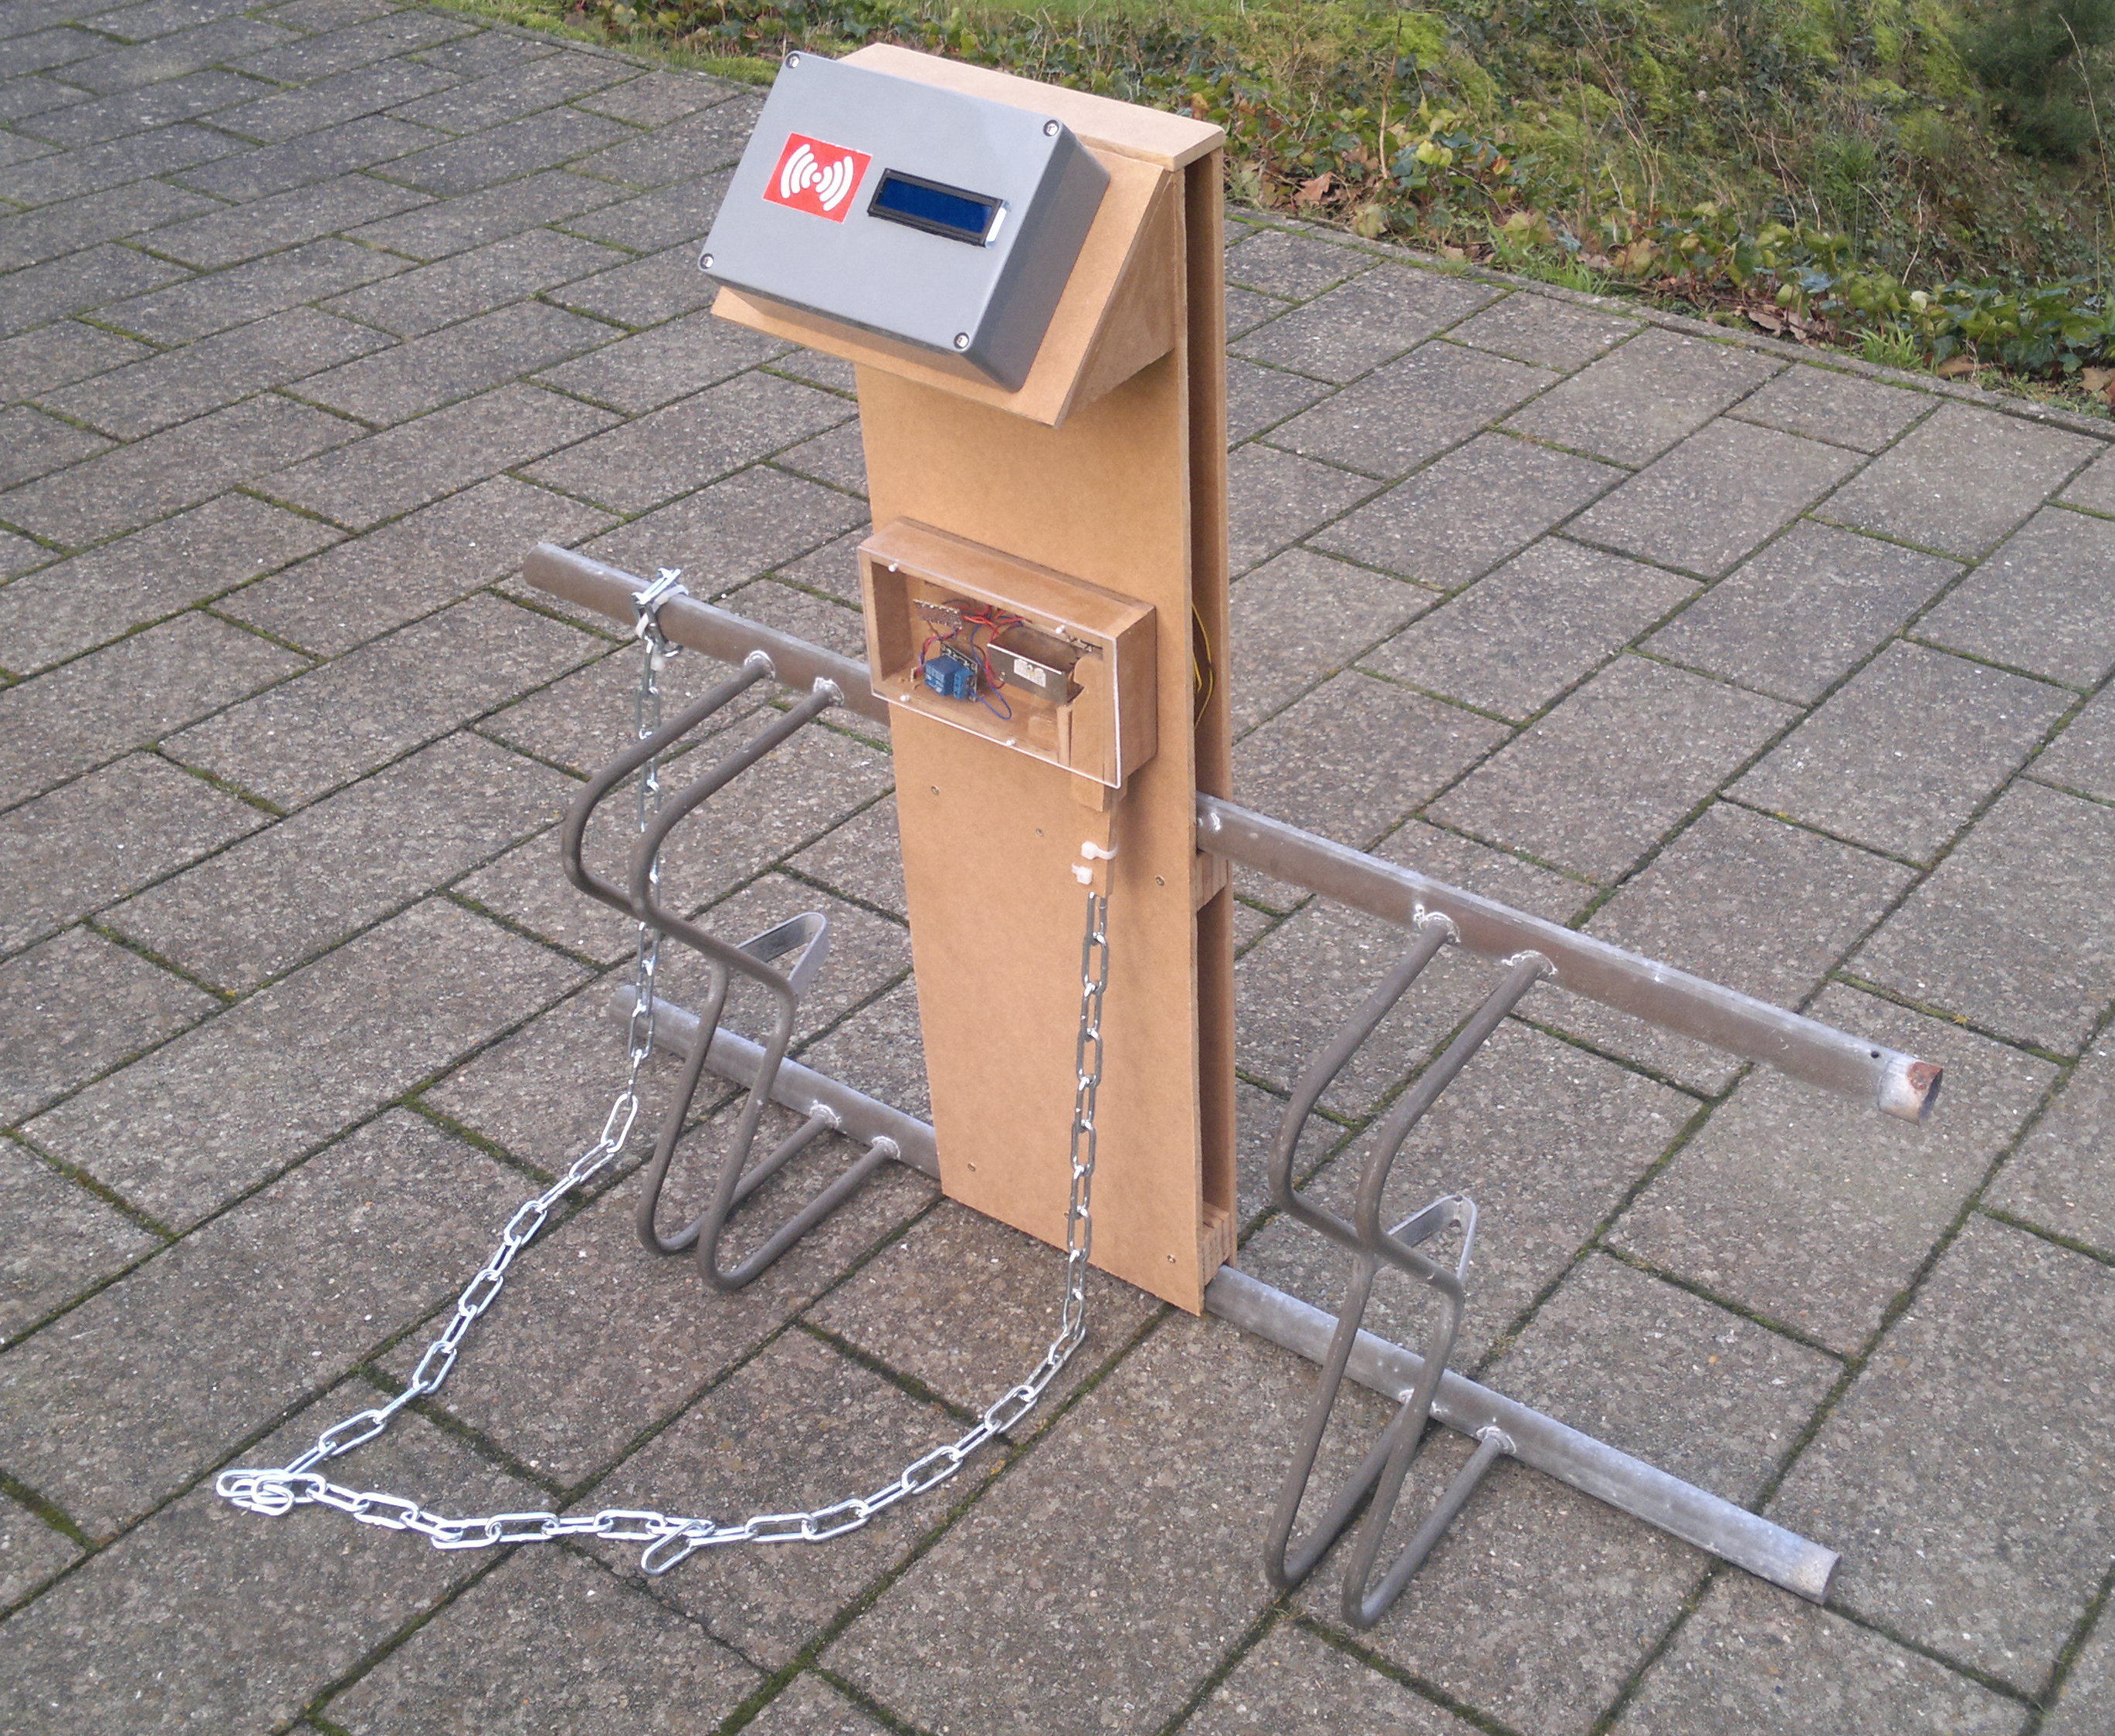
\includegraphics[width=0.6\textwidth]{images/desc/full.jpg}
	\caption{Picture of prototype rack}
	\label{fig.rack}
\end{figure}

The components in the main box are connected by plug-in cables and soldered where needed, according to our design. The lock case and the wall is made of plywood using basic tools. The lock case construction is glued and nailed together, built after a slightly altered design, due to the fact that more advanced tools were not available. 
